\documentclass{article}
\usepackage[utf8]{inputenc}
\usepackage{graphicx}
\usepackage[colorlinks=true, allcolors=black]{hyperref}
\usepackage{listings}
\usepackage[a4paper, total={6in, 8in}]{geometry}
\usepackage{pdfpages}
\usepackage{float}
\usepackage{soul}
\usepackage{multicol}
\usepackage{multirow}
\usepackage[section]{placeins}
\usepackage{subfig}
\usepackage[
backend=biber,
sorting=none]{biblatex}

\graphicspath{ {./img/} }

\addbibresource{bibliography.bib}

\lstset{
  basicstyle=\ttfamily,
  columns=fullflexible,
  breaklines=true,
}

\NewDocumentCommand{\codeword}{v}{%
\texttt{\textcolor{black}{#1}}%
}

\title{CS5011: P2 - Machine Learning}
\author{190018035}
\date{March 13th 2024}

% PAGE LIMIT: 10, including text, figures, tables

\begin{document}

\maketitle

\tableofcontents

\section{Introduction}
% Include checklist of parts completed & extension
For this practical, I was tasked with implementing and evaluating different machine learning models on the Pump It Up: Data Mining the Water Table \cite{DrivenData} dataset. The checklist below details my achievements in the practical for each of the specified parts.

\subsection{Project Achievements}
\begin{itemize}
    \item{Part 1: Attempted and Fully Working}
    \item{Part 2: Attempted and Fully Working}
\end{itemize}

\subsection{Usage Instructions}

To run the script, navigate to the root directory and run the following command:

\begin{lstlisting}[language=bash]
python3 part1.py <train-input-file> <train-labels-file> <test-input-file> <numerical-preprocessing> <categorical-preprocessing> <model-type> <test-prediction-output-file>
\end{lstlisting}

\noindent The values for each of the arguments are equivalent to that described in the assignment specification. However, one difference is that the \codeword{<numerical-preprocessing>} and \codeword{<categorical-preprocessing>} arguments now take in a \codeword{Manual} option, which allows features to be preprocessed based on the encoding that are most suitable for the feature. 

\section{Part 1}
In this section, I will detail the various preprocessing steps I took to prepare the data for the machine learning models.

\subsection{Preprocessing Steps}
Prior to implementing the machine learning models, I performed a number of preprocessing steps to clean and prepare the data for the models. These steps were guided by a deep exploration of the dataset, where I analyzed the distribution of the features, the relationships between the features, and other important characteristics of the dataset. In conjuction with the steps outlined below, I will also discuss my findings from the exploration that lead to the decisions I made.

\subsubsection{Cleaning the Data}
The following steps were taken to clean the data:

\paragraph{Removing Irrelevant Features}
The first step I took was to remove any features that were irrelevant to the prediction task. These features either did not directly contribute to the status of the water pumps or contained too many missing values. The features that were removed include:

\begin{itemize}
  \item \codeword{id} The identifier for the water pump is not relevant to the prediction task
  \item \codeword{wpt_name} The name of the water pump is unlikely to contribute to the prediction task
  \item \codeword{scheme_name} The name of the water scheme is unlikely to contribute to the prediction task
  \item \codeword{num_private} This feature contains mostly missing values, with over 99.24\% of the values missing (defined as 0). Additionally, the feature does not have a clear definition, so it is unclear how it would contribute to the prediction task.
  \item \codeword{amount_tsh} Similarly, this feature contains mostly missing values, with over 70.1\% of the values missing (also defined as 0). 
\end{itemize}

\paragraph{Removing Single-Value Features}
I also removed any features that only contained a single value, as they do not contribute to the prediction task. There was only one feature that met this criteria, which was \codeword{recorded_by}.

\paragraph{Removing Redundant Features}
There were a number of features that were redundant, meaning they contained the same information as another feature. I removed these features to reduce the dimensionality of the dataset. There were a few considerations I made when deciding which of the features that are redundant to remove. The first consideration was the cardinality of the feature - having too many unique values would make the feature difficult to encode, whilst having too few unique values would make the feature less informative. The second consideration was the number of missing values in the feature - if a feature had a large number of missing values, it would be less informative. The features that were removed include:

\begin{itemize}
  \item \codeword{payment} This feature contains the same information as \codeword{payment_type} with the same value counts, so I removed it and retained \codeword{payment_type}.
  \item \codeword{quantity} Similarly, this feature contains the same information as \codeword{quantity_group} with the same value counts, so I removed it and retained \codeword{quantity_group}.
  \item \codeword{extraction_type} This feaure was removed in favor of \codeword{extraction_type_group} and \\ \codeword{extraction_type_class}. The \codeword{extraction_type_class} feature provides a more general classification of the extraction type. It contains only 7 unique values, which makes it easier to encode, and the smallest value count for a given category for this feature is 117. The \codeword{extraction_type_group} feature, on the other hand, contains 13 unique values, where the smallest value count for a given category is 98. Finally, the \codeword{extraction_type} feature contains 18 unique values, where the smallest value count for a given category is 2. From this information, we can see that the \codeword{extraction_type_class} feature is the most general, and the \codeword{extraction_type} feature is the most specific, thereby providing a balance between the general and specific information provided to the model. 
  \item \codeword{scheme_management} This feature was removed in favor of \codeword{management}. These two features contain most of the same categories; however, the \codeword{scheme_management} feature contains 3878 missing/unknown values whereas management only contains 561 unknown values. This makes the \codeword{management} feature more informative and easier to encode.
  \item \codeword{water_quality} This feature was removed in favor of \codeword{quality_group}. These two features contain mostly the same information, where \codeword{water_quality} splits "salty" and "flouride" into two subcategories (introducing a "salty abandoned" and "flouride abandoned" subcategory). These subcategories contain comparatively few values, so I decided to remove the \codeword{water_quality} feature and retain the \codeword{quality_group} feature to reduce the dimensionality of the dataset.
  \item \codeword{source} This feature was removed in favor of \codeword{source_type} and \codeword{source_class}. The \codeword{source_class} feature is the most general, containing only 3 unique values, and the \codeword{source_type} feature sits in the middle, containing 7 unique values and containing very similar columns to \codeword{source}. The \codeword{source} feature contains 10 unique values. Since \codeword{source_class} provides the most general information, and since \codeword{source} contains the highest cardinality, I decided to remove the \codeword{source} feature and retain the other two so there is a balance between the general and specific information provided to the model.
  \item \codeword{waterpoint_type_group} This feature was removed in favor of \codeword{waterpoint_type}. The \\ \codeword{waterpoint_type} splits up the "communal standpipe" category into "communal standpipe" and "communal standpipe multiple". However, since "communal standpipe multiple" only contains contains relatively few values (6103), I decided to remove the \codeword{waterpoint_type_group} feature and retain the \codeword{waterpoint_type} feature to reduce the dimensionality of the dataset.
\end{itemize}

\paragraph{Replacing Construction Year with Decades}
The \codeword{construction_year} feature contained a large number of missing values, with 34.8\% of the values missing. To make the feature more informative, I decided to categorize the construction years into decades. This would allow the model to learn the relationship between the construction year and the status of the water pumps, without imputing values that might distort the underlying distribution of the data. The decades were defined from 1960s to the 2010s, with the missing values being replaced with the "Unknown" category.

\paragraph{Imputing Missing Values}
There were a number of numerical features that contained missing values, specifically \codeword{longitude}, \codeword{gps_height}, \codeword{population} and \codeword{district_code}. I wanted to avoid blindly imputing the missing values with the mean or median, as this could distort the underlying distribution of the data. Instead, I decided to impute the missing values using the mean of the feature grouped by the \codeword{region} feature. To ensure that this imputation method was valid, I ran a chi-squared test to check if the \codeword{region} feature was independent of the \codeword{longitude}, \codeword{gps_height}, \codeword{population} and \codeword{district_code} features. The results of the chi-squared test are shown in Table 1.

\begin{table}[H]
  \centering
\begin{tabular}{|c|c|c|c|}
\hline
                         & Chi2       & p-value                               & dof     \\ \hline
  \codeword{longitude} vs \codeword{region}      & 1187933.26 & 3.26e^{-133} & 1150320 \\ \hline
  \codeword{district_code} vs \codeword{region} & 119074.99  & 0                               & 360     \\ \hline
  \codeword{gps_height} vs \codeword{region}    & 531651.17  & 0                               & 48760   \\ \hline
  \codeword{population} vs \codeword{region}     & 457007.23  & 0                               & 21200   \\ \hline
\end{tabular}
\caption{Results of the chi-squared test between numerical features with missing values and the region feature}
\end{table}

\noindent The p-values for the chi-squared test were all less than 0.05, which indicates that the \codeword{region} feature is not independent of the above features. Therefore, I decided to impute the missing values using the mean of the feature grouped by the \codeword{region} feature, aside from \codeword{district_code}, where I used the median (to avoid floating point district codes). For categorical features, I replaced the missing values with the "Unknown" category, aside from the \codeword{permit} and \codeword{public_meeting} features, which I imputed using the mode of the feature due to the small number of missing values.

\paragraph{Fixing Formatting Issues}
When exploring the \codeword{funder} and \codeword{installer} features, I found that there were a large number of unique values, with some of the values being the same but formatted differently and consisting of spelling mistakes. For example, "tanzania government" and "tanzania\textit{n} government" were considered as two different unique values, and so was "regwa company of egypt" and "regwa company of \textit{egpty}". To address this, I first converted all the values to lowercase and then removed any leading/trailing whitespace. I then employed a fuzzy matching algorithm to group potentially duplicates based on a similarity threshold, which I set to 95\%. This threshold was determined through manual experimentation and set to a fairly high value to ensure that the algorithm didn't group values that were not duplicates. This approach helped consolidate the variations and reduce the cardinality of the features. Table 1 shows the reduction in the number of unique values for each of the features after fixing the formatting issues.

\begin{table}[H]
\centering
\begin{tabular}{|c|c|c|}
\hline
\textbf{Feature} & \textbf{Original Unique Values} & \textbf{Reduced Unique Values} \\ \hline
\codeword{funder} & 1896 & 1883 \\ \hline
\codeword{installer} & 2145 & 1905 \\ \hline
\end{tabular}
\caption{Reduction in unique values for high cardinality features when fixing formatting issues}
\end{table}

\paragraph{Limiting High Cardinality Features}
There were a few features in the dataset, specifically \codeword{funder}, \codeword{installer}, \codework{subvillage} and \codeword{ward}, that contained a large number of unique values. Such high cardinality could pose challenges, as encoding these features could significantly increase the dimensionality of the dataset, potentially leading to issues like overfitting and increased computational demand. To address this, I set a threshold (95\%) that identifies the most frequent categories that cumulatively account for 95\% of the values in the feature. This threshold was determined through manual experimentation, but can be set through hyperparameter optimization. Through this strategy, I was able to reduce the number of dummy variables needed for encoding and makng the dataset size more manageable. The remaining categories were replaced with the "Other" category. Additionally, I also replaced the missing values with the "Unknown" category. Table 2 details the following reductions in the number of unique values for each of the features (after fixing formatting issues):

\begin{table}[H]
\centering
\begin{tabular}{|c|c|c|}
\hline
\textbf{Feature} & \textbf{Original Unique Values} & \textbf{Reduced Unique Values} \\ \hline
\codeword{funder} & 1883 & 405 \\ \hline
\codeword{installer} & 1905 & 397 \\ \hline
\codeword{subvillage} & 19287 & 16336 \\ \hline
\codeword{ward} & 2092 & 1578 \\ \hline
\end{tabular}
\caption{Reduction in unique values for high cardinality features when applying the threshold of 95\%}
\end{table}

\paragraph{Converting Datetime Features}
The \codeword{date_recorded} feature was converted to a datetime object and then split into three separate features: \codeword{year}, \codeword{month}, and \codeword{day}. By doing so, I was able to extract the temporal information from the feature, which could be useful for the model to learn the relationship between the date the water pump was recorded and the functionality of the water pump. In Figure 1, we can see the distribution for each temporal feature. We can see that the year and month recorded display some seasonal trends, where certain months (e.g January, February, March) and certain years (e.g 2011, 2013) have a higher number of recorded water pumps. The day recorded, however, does not display any clear trends. When dropping the day recorded feature, however, the performance of the models did slightly decrease, so I decided to retain the feature.

\begin{figure}[H]
    \centering
    \subfloat[Distribution of the year recorded]{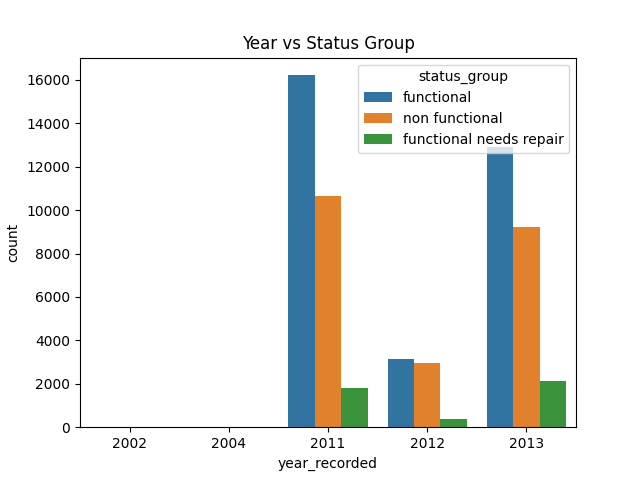
\includegraphics[width=0.35\textwidth]{img/year-vs-status_group.png}\label{fig:year_distribution}}
    \subfloat[Distribution of the month recorded]{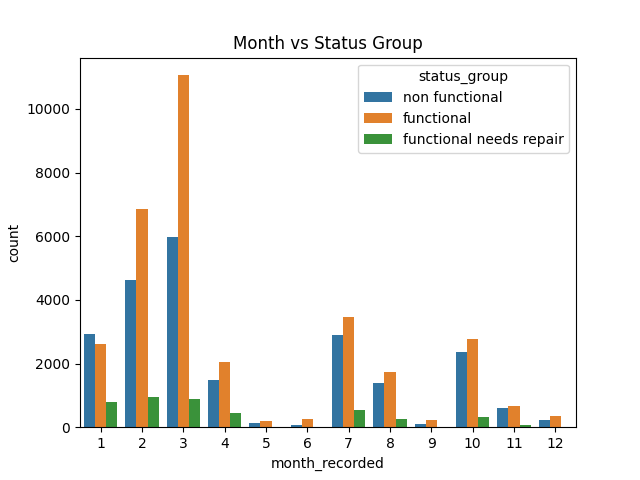
\includegraphics[width=0.35\textwidth]{img/month-vs-status_group.png}\label{fig:month_distribution}}
    \subfloat[Distribution of the day recorded]{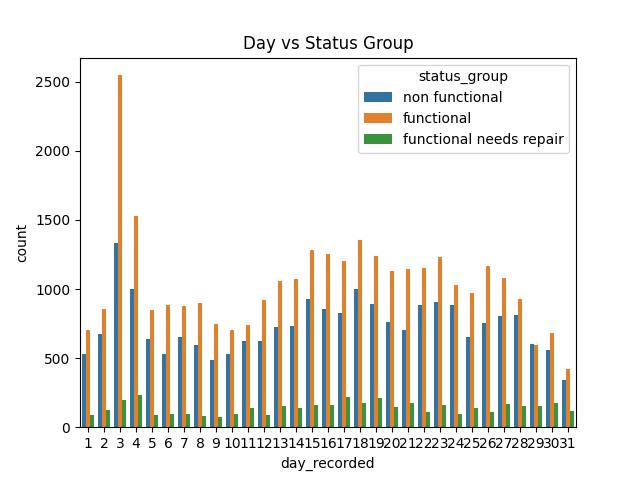
\includegraphics[width=0.35\textwidth]{img/day-vs-status_group.png}\label{fig:day_distribution}}
    \caption{Distribution of the date recorded with respect to the status of the water pump}
\end{figure}

\subsubsection{Encoding the Data}
In addition to the encoders specified in the assignment specification, I also implemented a \codeword{Manual} encoder, which allows features to be preprocessed based on the encoding that are most suitable for the feature. High-cardinality features were encoded using the Target Encoding method, and low-cardinality features were encoded using the One-Hot Encoding method. The only ordinal feature in the dataset, \codeword{decade}, was encoded using the Ordinal Encoding method. The numerical features that were encoded using the Standard Scaling method only included the \codeword{longitude}, \codeword{latitude}, \codeword{gps_height} and \codeword{population}.

\subsection{Design Decisions}
Before evaluating the performance of the models, I made a few design decisions to not only investigate its impact on the performance of the model, but also as a way to satisfy some of the data preprocessing requirements that each model has. These decisions are detailed below.

\subsubsection{Encoder Parameters}

There were two main parameters that I found to have an impact on the model's ability to run. For the One-Hot Encoding method, I set the \codeword{handle_unknown} parameter to "ignore" to avoid errors when the test set contains categories that were not present in the training set. I used a similar approach for the Target Encoding method, where I set the \codeword{handle_unknown} parameter to -1 for the same reason. 

\subsubsection{Model Parameters}
I wanted to investigate a few key hyperparameters for the Random Forest and HistGradientBoostingClassifier models. The default settings provide a strong baseline for the models, but I wanted to see the impact of changing some of the default parameter settings that significantly influence their performance. The parameters I chose for each model, along with the reasons for choosing them, are detailed below.

\paragraph{Random Forest}

\begin{itemize}
  \item \codeword{n_estimators} This is the number of trees in the forest. Investigating this parameter is crucial as more trees can improve the model's accuracy and robustness, at the cost of eventually plateauing and increasing the computational demands. For this reason, I set the \codeword{n_estimator}'s parameter to 200 (100 higher than the default) to see if the model's performance would improve.
  \item \codeword{max_depth} This is the maximum depth that the tree can grow. Investigating this parameter is crucial as a deeper tree can capture more complex patterns within the data, but can also lead to overfitting if it is too deep. The default value for this parameter is "None", which means that the tree will grow until all leaves are pure. I set the \codeword{max_depth} parameter to 20 to see if limiting the depth can reduce the risk of overfitting while still allowing the tree to capture complex patterns.
  \item \codeword{max_features} This parameter defines the number of features to consider when deciding upon a split. A value with a low parameter might not capture enough information for a strong prediction, while too high a value might lead to overfitting. I set the \codeword{max_features} parameter to "log2" (different from the default "sqrt") to see if taking the log of the number of features provides a better balance between capturing enough information and avoiding overfitting than the square root of the number of features.
\end{itemize}

\paragraph{HistGradientBoostingClassifier}

\begin{itemize}
  \item{\codeword{learning_rate}} This parameter shrinks the contribution of each tree to control the rate of learning. A low learning rate can lead to a more robust model, but at the cost of increased computational demands. I set the \codeword{learning_rate} parameter to 0.05 (different from the default 0.1) to see if a lower learning rate can improve the model's robustness.
  \item{\codeword{min_samples_leaf}} This parameter is the minimum number of samples required to be at a leaf node. A higher value forces the model to make a split only if there are enough samples to populate the leaf, which deters the model from making splits that capture noise. I increased the \codeword{min_samples_leaf} parameter to 100 (different from the default 20) to see if a higher values avoids the model from capturing noise.

\end{itemize}

\subsection{Evaluation}
To evaluate the performance of each model, I ran a 5-fold cross-validation on the training set. I experimented with different preprocessing encodings, including Standard Scaling (SS) and Passthrough (PT) for the numerical features, and One-Hot Encoding (OHE), Ordinal Encoding (Ord), and Target Encoding (Target) for the categorical features. The models where ran with the default hyper-parameters. The results of the experiments are shown in the Table 4 below.

\begin{table}[H]
  {\footnotesize
  \begin{tabular}{|c|c|c|c|c|c|c|}
    \hline
    \textbf{}              & SS + OHE & SS + Ord & SS + Target & PT + OHE & PT + Ord & PT + Target \\ \hline
    \codeword{RandomForestClassifier}          & 80.74\%  & 80.79\%  & 80.4\%      & 80.2\%   & 79.09\%  & 79.85\%     \\ \hline
    \codeword{LogisticRegression}    & 78.49\%  & 62.24\%  & 75.52\%     & 78.37\%  & 61.44\%  & 75.53\%     \\ \hline
    \codeword{GradientBoostingClassifier}      & 75.96\%  & 75.16\%  & 77.53\%     & 75.71\%  & 74.56\%  & 74.56\%     \\ \hline
    \codeword{HistGradientBoostingClassifier} & 79.39\%  & 79.12\%  & 79.62\%     & 78.67\%  & 78.37\%  & 78.89\%     \\ \hline
    \codeword{MLPClassifier}                    & 77.59\%  & 53.36\%  & 78.16\%     & 77.54\%  & 54.33\%  & 77.7\%      \\ \hline
  \end{tabular}
}
  \caption{Results of each model with different preprocessing encodings}
\end{table}

\subsubsection{General Observations}
This section will cover some key findings from the experiments with each model on default hyper-parameters and different preprocessing encodings.

\paragraph{Random Forest}
Random Forest performed the best out of all the models, with the best accuracy of 80.79\% using Standard Scaling and Ordinal Encoding. This could be attributed to the model's inherent robustness to feature scaling and the ability to handle categorical features. It is possible that ordinal encoding provides a more meaningful way to represent categorical features than other types of preprocessing without increasing the dimensionality too much, aligning with Random Forest's capacity to manage features with high cardinality. However, we do see that scaling the numerical features does have a significant impact, since ordinal encoding performed the worst out of all the combinations when using the passthrough encoding. 

\paragraph{Logistic Regression}
Logistic Regression performed the best when using One-Hot Encoding. This could be because one hot encoding ensures linear independence for each feature, whereas ordinal encoding might introduce some form of ordinality that might not be present in the data and target encoding might introduce some form of leakage. For this same reason, this may be why the model performed the worst when using ordinal encoding, as there is a clear violation of the assumption of linear independence.

\paragraph{Gradient Boosting Classifier}
Gradient Boosting Classifier performed best when target encoding is applied. This could be due to the model's gradient boosting mechanism. Target encoding could help reduce overfitting by smoothing out the effect of the rare categories, which is crucial for gradient boosting models. Additionally, since the model is tree-based, it can inherently handle categorical features, which aligns with the target encoding method.

\paragraph{HistGradientBoostingClassifier}
Across all models, HistGradientBoostingClassifier performed second best. There is a significant improvement in the model's performance when using standard scaling, as the accuracies are consistently higher than when using passthrough. This could be due to the model's ability to handle different scales in numerical features. By utilizing Standard Scaling, this might help in the model's ability to learn the relationships between the features and the target variable.

\paragraph{MLP Classifier}
One notable observation is that MLPClassifier performs the worst when using ordinal encoding. This could be due to the model's reliance on gradient-based optimization which can be sensitive to feature scaling. Since ordinal encoding exacts an ordinality that might not be present in the data, this could potentially confuse the model and lead to poor performance.

\subsubsection{Random Forest with Parameter Setting}
Below are the results of the Random Forest model with different hyper-parameters using Standard Scaling and Ordinal Encoding. Each parameter was tested on its own to see the impact on the model's default performance. The results are shown in Table 5. 

\begin{table}[H]
  \centering
\begin{tabular}{|c|c|c|c|}
\hline
Default & n\_esimators & max\_depth & max\_features \\ \hline
80.79\% & 80.81\%      & 80.82\%    & 80.80\%       \\ \hline
\end{tabular}
\caption{Results of Random Forest with different hyper-parameters using Standard Scaling and OrdinalEncoder}
\end{table}

\noindent From these results, we can make a few observations. Firstly, by increasing the number of trees, the model's performance slightly improves. This is expected, as more trees can improve the model's accuracy and robustness. Limiting the depth of the tree also slightly improves the model's performance, signalling that the default tree depth might be too deep and is leading to overfitting. Finally, taking the log of the number of features as opposed to the default method of square rooting the number of features also slightly improves the model's performance. This could be due to the log leading to a more balanced consideration of feature importance across the trees, improving the generalization of the model.

\subsubsection{HistGradientBoostingClassifier with Parameter Setting}

\begin{table}[H]
  \centering
  \begin{tabular}{|c|c|c|}
    \hline
    Default & learning\_rate & min\_samples\_leaf \\ \hline
    79.62\% & 79.24\%        & 79.64\%            \\ \hline
  \end{tabular}
  \caption{Results of HistGradientBoostingClassifier with different hyper-parameters using Standard Scaling and TargetEncoder}
\end{table}

\section{Part 2}
% Analyse the results of your experiments based on the provided training set (via cross-
% validation mechanism). Summarise the key insights and findings of your analysis.
For this part of the practical, I utilized Optuna \cite{optuna_2019}, an automated hyper-parameter optimization (HPO) tool to find the best hyper-parameters for each of the models. In this section, I will detail my HPO process and analyze the results of the experiments.

% TODO REDO
\subsection{Hyper-Parameter Optimization}
I decided to use Optuna to perform the hyper-parameter optimization for the Random Forest and Logistic Regression models. I chose Random Forest as from the previous part, it was the best performing model, and Logistic Regression as it is a simple model that can be used as a benchmark. I also wanted to see how HPO differs for different families of models. The hyper-parameters that I optimized for each of the models are detailed below.

% TODO REDO
\subsubsection{Random Forest}
When running the study for the Random Forest model, I optimized the following hyper-parameters:

\begin{itemize}
  \item \codeword{n_estimators} The number of trees in the forest
  \item \codeword{max_depth} The maximum depth of the tree
  \item \codeword{min_samples_split} The minimum number of samples required to split an internal node
  \item \codeword{min_samples_leaf} The minimum number of samples required to be at a leaf node
  \item \codeword{max_features} The number of features to consider when looking for the best splits
\end{itemize}

% TODO REDO
\subsubsection{Logistic Regression}
When running the study for the Logistic Regression model, I optimized the following hyper-parameters:

\begin{itemize}
  \item \codeword{C} Inverse of regularization strength
  \item \codeword{penalty} The norm used in the penalization
  \item \codeword{solver} The algorithm to use in the optimization problem
  \item \codeword{class_weight} Weights associated with classes in the form \{class\_label: weight\}
  \item \codeword{tol} Maximum number of iterations taken for the solvers to converge
  \item \codeword{max_iter} Maximum number of iterations taken for the solvers to converge
\end{itemize}

\subsection{Evaluation}



\subsubsection{Random Forest}
When running the trials, I found that the most important hyper-parameters for the Random Forest model were \codeword{cat_encoder}, \codeword{max_depth}, and \codeword{max_features}. These parameters were the most influential in determining the performance of the model. 

\begin{figure}[H]
  \centering
  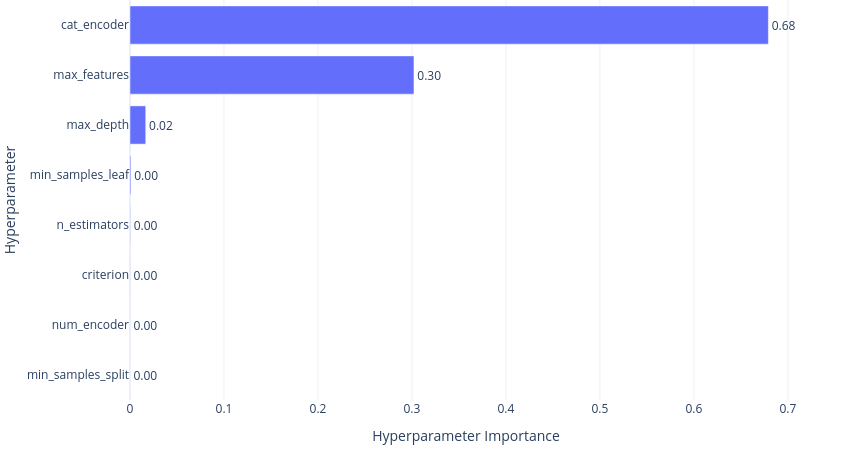
\includegraphics[width=0.5\textwidth]{img/random_forest_importance.png}
  \caption{Feature Importance for Random Forest Model}
\end{figure}

\noindent In addition, the parallel coordinates plot for the Random Forest model for the most influential features is shown below.

\begin{figure}[H]
  \centering
  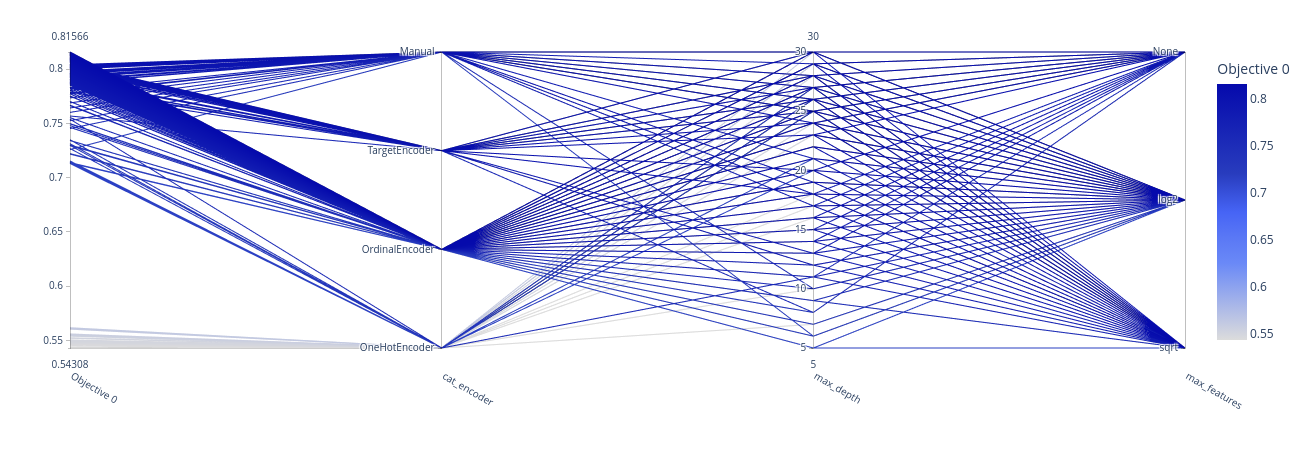
\includegraphics[width=0.5\textwidth]{img/tmp.png}
  \caption{Parallel Coordinates Plot for Random Forest Model}
\end{figure}

\subsubsection{Logistic Regression}
When running the trials, I found that the most important hyper-parameters for the Logistic Regression model were \codeword{cat_encoder}, \codeword{solver}, and \codeword{class_weight}. These parameters were the most influential in determining the performance of the model.

\begin{figure}[H]
  \centering
  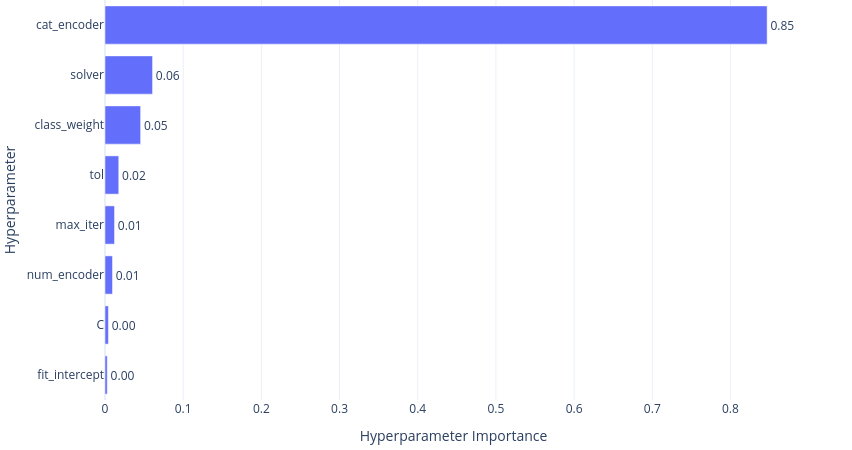
\includegraphics[width=0.5\textwidth]{img/lr_importance.png}
  \caption{Feature Importance for Logistic Regression Model}
\end{figure}

\noindent In addition, the parallel coordinates plot for the Logistic Regression model for the most iinfluencial features is shown below.

\begin{figure}[H]
  \centering
  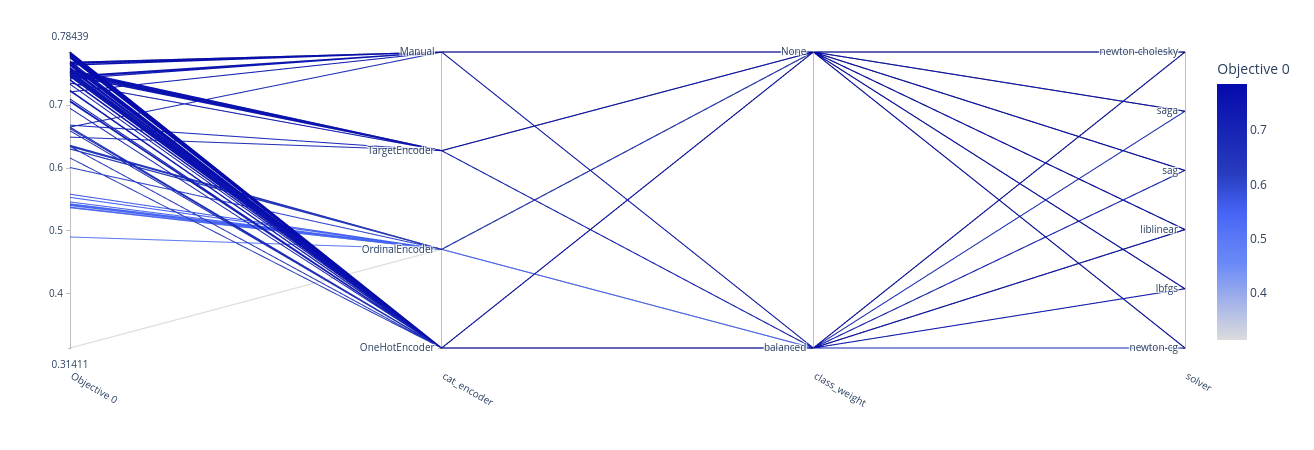
\includegraphics[width=0.5\textwidth]{img/tmp2.png}
  \caption{Parallel Coordinates Plot for Logistic Regression Model}
\end{figure}

\section{Conclusion}
In this practical, I implemented and evaluated different machine learning models on the Pump It Up: Data Mining the Water Table dataset. I performed a number of preprocessing steps to clean and prepare the data for the models, and made a few design decisions to investigate its impact on the performance of the model. I also utilized Optuna to perform the hyper-parameter optimization for the Random Forest and Logistic Regression models. When submitting the predictions to the competition, I achieved an accuracy of 82.36\% on the test set using the tuned RandomForestClassifier, which placed me at \#823 on the leaderboard.

\begin{figure}[H]
  \centering
  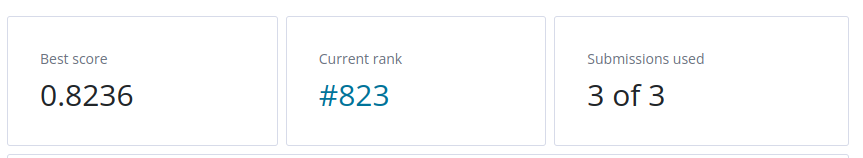
\includegraphics[width=0.8\textwidth]{img/leaderboard.png}
  \caption{Test set accuracy and leaderboard position}
\end{figure}

\printbibliography

\end{document}
